\begin{solution}

\begin{enumerate}
\item The error is shown in the table below.  The plot is shown with the
      solution to part~(c).  The code that generated this plot follows 
      at the end of the problem.
\begin{center}
\begin{tabular}{rr}
\hline
\multicolumn{1}{c}{$N$} & \multicolumn{1}{c}{error} \\ 
\hline
   2  &  2.2920610 \\
   4  &  1.2480270 \\
   8  &  0.6514086 \\
  16  &  0.3327167 \\
  32  &  0.1681236 \\
  64  &  0.0845039 \\
 128  &  0.0423625 \\
 256  &  0.0212089 \\
 512  &  0.0106114
\end{tabular}\end{center} 

\item The $O(h^2)$ centered difference approximation gives
\begin{center}
\begin{tabular}{rr}
\hline
\multicolumn{1}{c}{$N$} & \multicolumn{1}{c}{error} \\
\hline
   2 &  0.4117528 \\
   4 &  0.1461393 \\
   8 &  0.0448560 \\
  16 &  0.0125498 \\
  32 &  0.0033288 \\
  64 &  0.0008579 \\
 128 &  0.0002178 \\
 256 &  0.0000549 \\
 512 &  0.0000138
\end{tabular}\end{center}
These errors decay much more rapidly than for the analogous expansion in part~(a).
This is made clear by the plot below, generated by the following code.

\item Roughly speaking, the forward difference requires $N\approx 512$ 
before it is accurate to two digits, while the centered difference only requires 
$N\approx 16$.   (When used in the context of solving differential equations,
the improved accuracy of the centered difference formula allows one to work
with smaller matrices than required for the forward difference formula,
potentially delivering a great speed-up in run-time.)

\begin{center}
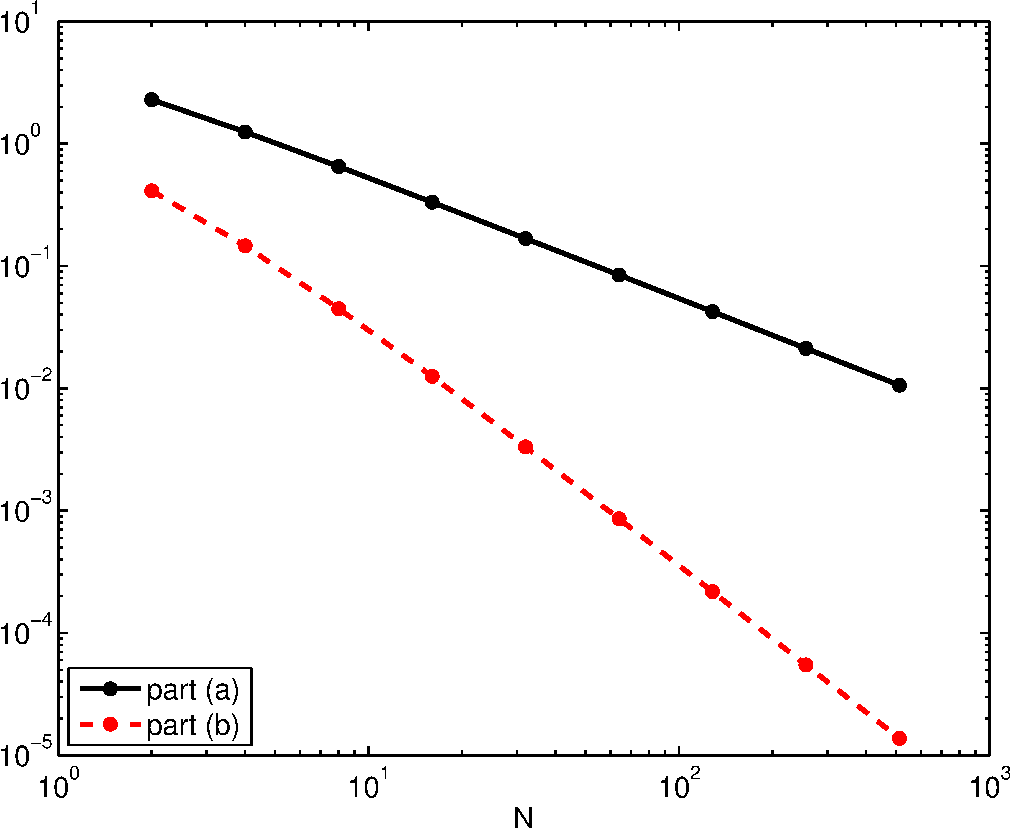
\includegraphics[scale=0.7]{findiff}
\end{center}

{\small \begin{verbatim}
 u = inline('exp(2*x)');
 uprime = inline('2*exp(2*x)');

 Nvec = 2.^[1:9]';
 err = zeros(size(Nvec));
 x = 1/2;
 fprintf('\n part (a)\n')
 for k=1:length(Nvec)
    N = Nvec(k);
    h = 1/(N+1);
    deriv = (u(x+h)-u(x))/h;
    err(k) = abs(uprime(x)-deriv);
    fprintf(' %3d   %10.7f\n', N, err(k));
 end
 loglog(Nvec,err,'k.-','linewidth',2,'markersize',20)

 fprintf('\n part (b)\n')
 for k=1:length(Nvec)
    N = Nvec(k);
    h = 1/(N+1);
    deriv = (u(x+h)-u(x-h))/(2*h);
    err(k) = abs(uprime(x)-deriv);
    fprintf(' %3d   %10.7f\n', N, err(k));
 end
 hold on
 loglog(Nvec,err,'r--','linewidth',2,'marker','.','markersize',20)
 set(gca,'fontsize',14)
 xlabel('N', 'fontsize',14)
 legend('part (a)','part (b)',3)
 print -depsc2 findiff.eps
\end{verbatim}}

\item Adding together the Taylor expansions 
\begin{align*}
u(x+h) &= u(x) + u'(x)h + \frac{u''(x)}{2}h^2 + \frac{u'''(x)}{3!}h^3 + \ldots\\
u(x-h) &= u(x) - u'(x)h + \frac{u''(x)}{2}h^2 - \frac{u'''(x)}{3!}h^3 + \ldots
\end{align*}
gives 
\[
u(x+h) + u(x-h) = 2u(x) + u''(x)h^2 + 2\frac{u''''(x)}{4!}h^4 + \ldots.
\]
Subtracting $2u(x)$ from both sides and dividing by $h^2$ gives
\[
\frac{u(x+h) -2u(x) + u(x-h)}{h^2} = u''(x) + 2\frac{u''''(x)}{4!}h^2 + \ldots,
\]
implying that the truncation error decreases at the same rate that $h^2$ decreases (if $h$ is small enough).  This implies the 2nd order central finite difference formula is $O(h^2)$ accurate.  

\end{enumerate}

%Bonus problem.  
%
%[\textbf{GRADERS}: please only award bonus credit for students
%who get this problem entirely correct: no partial credit on the bonus.]
%
%By manipulation of Taylor series, one arrives at the expansion
%\[ u'(x_0) = {-3 u(x_0) + 4 u(x_1) - u(x_2) \over 2 h} + O(h^2),\]
%i.e., $\alpha = -3/(2h)$, $\beta = 2/h$, and $\gamma = -1/(2h)$.
%
%On the other end of the domain, one has
%\[ u'(x_{N+1}) = {u(x_{N-1}) - 4 u(x_N) + 3 u(x_{N+1}) \over 2 h} + O(h^2).\]

\end{solution}
